
\documentclass[letterpaper,hide notes,xcolor={table,svgnames},pdftex,10pt]{beamer}
\def\showexamples{t}

\usecolortheme{crane}
\setbeamertemplate{navigation symbols}{}

\usetheme{MyPittsburgh}
\usepackage{hyperref}
\usepackage{graphicx,xspace}
\usepackage[normalem]{ulem}
\usepackage{multicol}
\usepackage{amsmath,amssymb,amsthm,graphicx,xspace}
\newcommand\SF[1]{$\bigstar$\footnote{SF: #1}}

\usepackage[sfdefault,lf]{carlito}
\usepackage[T1]{fontenc}
\usepackage[scaled]{beramono}
\usepackage{tikzpagenodes}
\newcommand{\Rplus}{\protect\hspace{-.1em}\protect\raisebox{.35ex}{\small{\small\textbf{+}}}}
\newcommand{\Cpp}{\mbox{C\Rplus\Rplus}\xspace}

\newcounter{tmpnumSlide}
\newcounter{tmpnumNote}

\newcommand\mnote[1]{%
	\addtocounter{tmpnumSlide}{1}
	\ifdefined\showcues {~\tiny\fbox{\arabic{tmpnumSlide}}}\fi
	\note{\setlength{\parskip}{1ex}\addtocounter{tmpnumNote}{1}\textbf{\Large \arabic{tmpnumNote}:} {#1\par}}}

\newcommand\mmnote[1]{\note{\setlength{\parskip}{1ex}#1\par}}


\newcommand\mquestion[2]{{~\color{red}\fbox{?}}\note{\setlength{\parskip}{1ex}\par{\Large \textbf{?}} #1} \note{\setlength{\parskip}{1ex}\par{\Large \textbf{A}} #2\par}\ifdefined \presentationonly \pause \fi}

\newcommand\blackboard[1]{%
	\ifdefined   \showblackboard
		{#1}
	\else {\begin{center} \fbox{\colorbox{blue!30}{%
						\begin{minipage}{.95\linewidth}%
							\hspace{\stretch{1}} Some space intentionally left blank; done at the blackboard.%
						\end{minipage}}}\end{center}}%
	\fi%
}

\usepackage{listings}
\lstset{%
	keywordstyle=\bfseries,
	aboveskip=15pt,
	belowskip=15pt,
	captionpos=b,
	identifierstyle=\ttfamily,
	frame=lines,
	numbers=left, basicstyle=\scriptsize, numberstyle=\tiny, stepnumber=0, numbersep=2pt}

\usepackage{siunitx}
\newcommand\sius[1]{\num[group-separator = {,}]{#1}\si{\micro\second}}
\newcommand\sims[1]{\num[group-separator = {,}]{#1}\si{\milli\second}}
\newcommand\sins[1]{\num[group-separator = {,}]{#1}\si{\nano\second}}
\sisetup{group-separator = {,}, group-digits = true}

%% -------------------- tikz --------------------
\usepackage{tikz}
\usetikzlibrary{positioning}
\usetikzlibrary{arrows,backgrounds,automata,decorations.shapes,decorations.pathmorphing,decorations.markings,decorations.text}

\tikzstyle{place}=[circle,draw=blue!50,fill=blue!20,thick, inner sep=0pt,minimum size=6mm]
\tikzstyle{transition}=[rectangle,draw=black!50,fill=black!20,thick, inner sep=0pt,minimum size=4mm]

\tikzstyle{block}=[rectangle,draw=black, thick, inner sep=5pt]
\tikzstyle{bullet}=[circle,draw=black, fill=black, thin, inner sep=2pt]

\tikzstyle{pre}=[<-,shorten <=1pt,>=stealth',semithick]
\tikzstyle{post}=[->,shorten >=1pt,>=stealth',semithick]
\tikzstyle{bi}=[<->,shorten >=1pt,shorten <=1pt, >=stealth',semithick]

\tikzstyle{mut}=[-,>=stealth',semithick]

\tikzstyle{treereset}=[dashed,->, shorten >=1pt,>=stealth',thin]

\usepackage{ifmtarg}
\usepackage{xifthen}
\makeatletter
% new counter to now which frame it is within the sequence
\newcounter{multiframecounter}
% initialize buffer for previously used frame title
\gdef\lastframetitle{\textit{undefined}}
% new environment for a multi-frame
\newenvironment{multiframe}[1][]{%
	\ifthenelse{\isempty{#1}}{%
		% if no frame title was set via optional parameter,
		% only increase sequence counter by 1
		\addtocounter{multiframecounter}{1}%
	}{%
		% new frame title has been provided, thus
		% reset sequence counter to 1 and buffer frame title for later use
		\setcounter{multiframecounter}{1}%
		\gdef\lastframetitle{#1}%
	}%
	% start conventional frame environment and
	% automatically set frame title followed by sequence counter
	\begin{frame}%
		\frametitle{\lastframetitle~{\normalfont(\arabic{multiframecounter})}}%
		}{%
	\end{frame}%
}
\makeatother

\makeatletter
\newdimen\tu@tmpa%
\newdimen\ydiffl%
\newdimen\xdiffl%
\newcommand\ydiff[2]{%
	\coordinate (tmpnamea) at (#1);%
	\coordinate (tmpnameb) at (#2);%
	\pgfextracty{\tu@tmpa}{\pgfpointanchor{tmpnamea}{center}}%
	\pgfextracty{\ydiffl}{\pgfpointanchor{tmpnameb}{center}}%
	\advance\ydiffl by -\tu@tmpa%
}
\newcommand\xdiff[2]{%
	\coordinate (tmpnamea) at (#1);%
	\coordinate (tmpnameb) at (#2);%
	\pgfextractx{\tu@tmpa}{\pgfpointanchor{tmpnamea}{center}}%
	\pgfextractx{\xdiffl}{\pgfpointanchor{tmpnameb}{center}}%
	\advance\xdiffl by -\tu@tmpa%
}
\makeatother
\newcommand{\copyrightbox}[3][r]{%
	\begin{tikzpicture}%
		\node[inner sep=0pt,minimum size=2em](ciimage){#2};
		\usefont{OT1}{phv}{n}{n}\fontsize{4}{4}\selectfont
		\ydiff{ciimage.south}{ciimage.north}
		\xdiff{ciimage.west}{ciimage.east}
		\ifthenelse{\equal{#1}{r}}{%
			\node[inner sep=0pt,right=1ex of ciimage.south east,anchor=north west,rotate=90]%
			{\raggedleft\color{black!50}\parbox{\the\ydiffl}{\raggedright{}#3}};%
		}{%
			\ifthenelse{\equal{#1}{l}}{%
				\node[inner sep=0pt,right=1ex of ciimage.south west,anchor=south west,rotate=90]%
				{\raggedleft\color{black!50}\parbox{\the\ydiffl}{\raggedright{}#3}};%
			}{%
				\node[inner sep=0pt,below=1ex of ciimage.south west,anchor=north west]%
				{\raggedleft\color{black!50}\parbox{\the\xdiffl}{\raggedright{}#3}};%
			}
		}
	\end{tikzpicture}
}


%% --------------------

%\usepackage[excludeor]{everyhook}
%\PushPreHook{par}{\setbox0=\lastbox\llap{MUH}}\box0}

%\vspace*{\stretch{1}

%\setbox0=\lastbox \llap{\textbullet\enskip}\box0}

\setlength{\parskip}{\fill}

\newcommand\noskips{\setlength{\parskip}{1ex}}
\newcommand\doskips{\setlength{\parskip}{\fill}}

\newcommand\xx{\par\vspace*{\stretch{1}}\par}
\newcommand\xxs{\par\vspace*{2ex}\par}
\newcommand\tuple[1]{\langle #1 \rangle}
\newcommand\code[1]{{\sf \footnotesize #1}}
\newcommand\ex[1]{\uline{Example:} \ifdefined \presentationonly \pause \fi
	\ifdefined\showexamples#1\xspace\else{\uline{\hspace*{2cm}}}\fi}

\newcommand\ceil[1]{\lceil #1 \rceil}


\AtBeginSection[]
{
	\begin{frame}
		\frametitle{Outline}
		\tableofcontents[currentsection]
	\end{frame}
}



\pgfdeclarelayer{edgelayer}
\pgfdeclarelayer{nodelayer}
\pgfsetlayers{edgelayer,nodelayer,main}

\tikzstyle{none}=[inner sep=0pt]
\tikzstyle{rn}=[circle,fill=Red,draw=Black,line width=0.8 pt]
\tikzstyle{gn}=[circle,fill=Lime,draw=Black,line width=0.8 pt]
\tikzstyle{yn}=[circle,fill=Yellow,draw=Black,line width=0.8 pt]
\tikzstyle{empty}=[circle,fill=White,draw=Black]
\tikzstyle{bw} = [rectangle, draw, fill=blue!20,
text width=4em, text centered, rounded corners, minimum height=2em]

\newcommand{\CcNote}[1]{% longname
	This work is licensed under the \textit{Creative Commons #1 3.0 License}.%
}
\newcommand{\CcImageBy}[1]{%
	\includegraphics[scale=#1]{creative_commons/cc_by_30.pdf}%
}
\newcommand{\CcImageSa}[1]{%
	\includegraphics[scale=#1]{creative_commons/cc_sa_30.pdf}%
}
\newcommand{\CcImageNc}[1]{%
	\includegraphics[scale=#1]{creative_commons/cc_nc_30.pdf}%
}
\newcommand{\CcGroupBySa}[2]{% zoom, gap
	\CcImageBy{#1}\hspace*{#2}\CcImageNc{#1}\hspace*{#2}\CcImageSa{#1}%
}
\newcommand{\CcLongnameByNcSa}{Attribution-NonCommercial-ShareAlike}

\newenvironment{changemargin}[1]{% 
	\begin{list}{}{% 
		\setlength{\topsep}{0pt}% 
		\setlength{\leftmargin}{#1}% 
		\setlength{\rightmargin}{1em}
		\setlength{\listparindent}{\parindent}% 
		\setlength{\itemindent}{\parindent}% 
		      \setlength{\parsep}{\parskip}% 
		      }% 
		\item[]}{\end{list}}




\title{Lecture 24 --- Reliability: RAID }

\author{Jeff Zarnett \\ \small \texttt{jzarnett@uwaterloo.ca}}
\institute{Department of Electrical and Computer Engineering \\
  University of Waterloo}
\date{\today}


\begin{document}

\begin{frame}
  \titlepage

 \end{frame}


\begin{frame}
\frametitle{Failure is Always an Option}

\begin{center}
	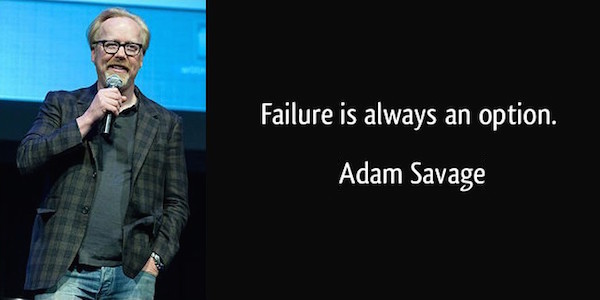
\includegraphics[width=0.75\textwidth]{images/failure.jpg}
\end{center}

Sometimes hard drives die -- so now what?

\end{frame}


\begin{frame}
\frametitle{Backups}

Backups help but they are not the only way.

A backup may be a bit out of date?

Are you sure they work?

\end{frame}


\begin{frame}
\frametitle{Now What?}

\begin{center}
	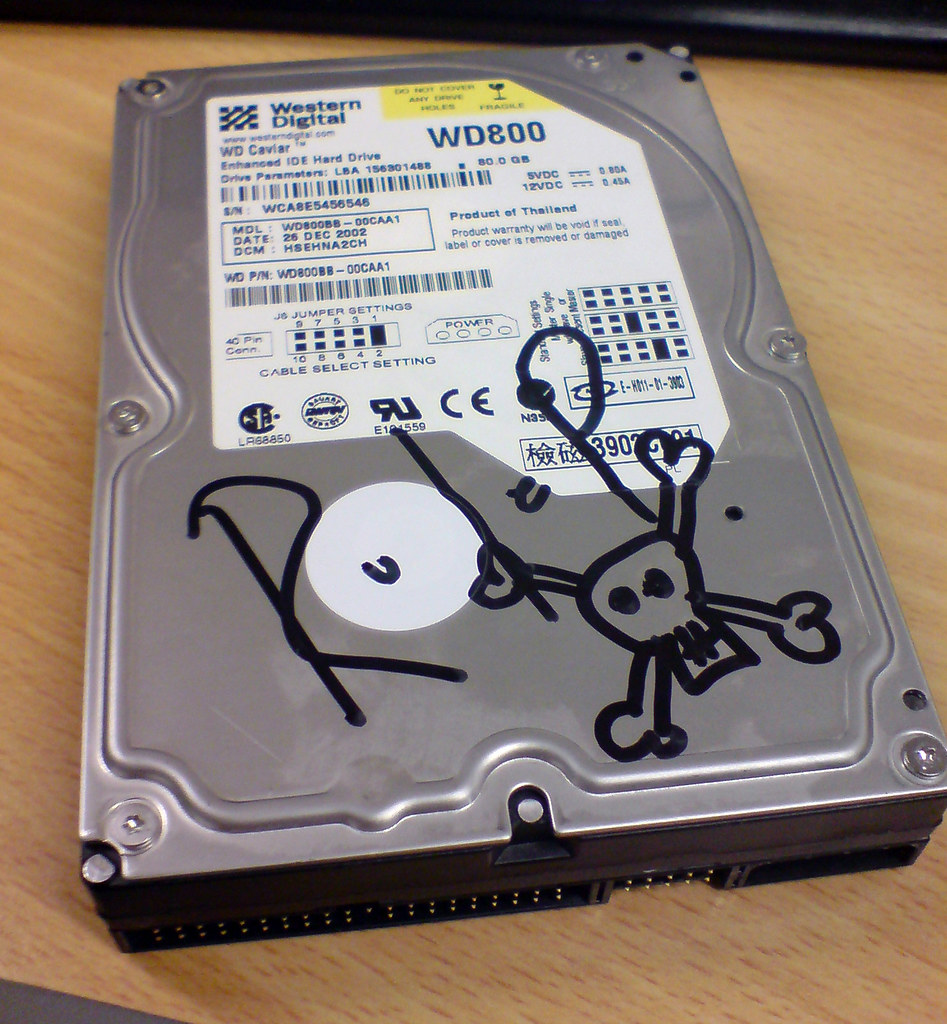
\includegraphics[width=0.5\textwidth]{images/rip-hdd.jpg}
\end{center}

Maybe loss of data, maybe system is down, maybe reduced performance?

\end{frame}


\begin{frame}
\frametitle{Too Good To Be True?}

 What if I told you there exists a solution to this where you not only get higher reliability and availability, but also maybe better performance?

\begin{center}
	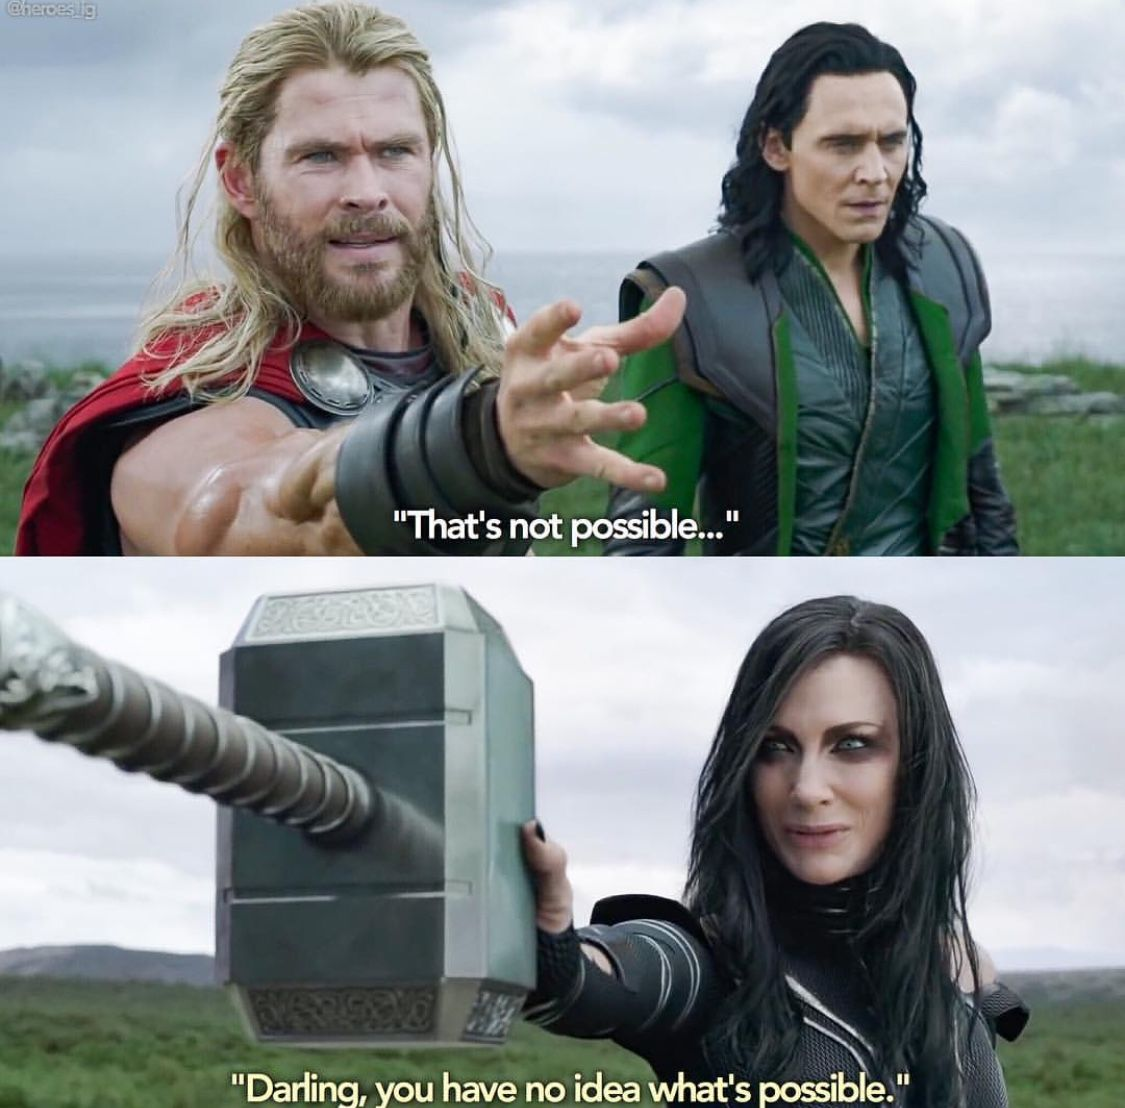
\includegraphics[width=0.4\textwidth]{images/hela.jpg}
\end{center}

It does cost money... But it's not magic.

\end{frame}


\begin{frame}
\frametitle{The Solution is Called...}

\begin{center}
	
\includegraphics[width=\textwidth]{images/raid.jpg}
\end{center}

\end{frame}

\begin{frame}
\frametitle{The Solution is Called...}

\begin{center}
	
\includegraphics[width=\textwidth]{images/leo.jpg}
\end{center}

\end{frame}


\begin{frame}
\frametitle{RAID}

RAID: Redundant Array of Independent Disks.


Multiple different independent disks that work together but appear to the user as if they are one drive/volume.

Can be managed in software or hardware.

\end{frame}


\begin{frame}
\frametitle{How Much Redundancy?}

Choose level of redundancy based on the data in question.

Is losing data inconvenient? A tragedy? Does it affect uptime?

\end{frame}


\begin{frame}
\frametitle{MttF}

For any device we can talk about the \alert{mean time to failure}.

This is always an estimate!

\begin{center}
	
\includegraphics[width=0.5\textwidth]{images/keanu.jpg}
\end{center}

\end{frame}


\begin{frame}
\frametitle{MttF Math}

Let's say you bought a disk that says its mean time to failure is 100~000 hours (11.4 years)

You might think that this is perfectly fine, even if it lives only half its expected life it's still more than five years and you'll replace it by then!

... but if you are running a data centre and you have 100 of them, the MttF of one of these disks is really only 100~000 / 100 = 1~000 hours (41.66 days).

\end{frame}


\begin{frame}
\frametitle{Another One Bites the Dust}

The textbook example is misleading -- hard drive deaths aren't evenly distributed!

It's more likely that everything is fine for a while and then drives start dying in quick succession. 


\end{frame}


\begin{frame}
\frametitle{No Free Lunch}

So if we want to have improved reliability, it's obvious this is going to have a cost. 

The cost is in the redundancy; having more than one copy of the data and those copies are stored on different physical storage media.

Either: more money for more disks, or less total capacity for more redundancy.

\end{frame}


\begin{frame}
\frametitle{Mirroring}

Obvious approach is \alert{mirroring}.

If one of the disks dies, then the data is on the other disk and it's not lost.


How fast do we have to replace it?
\end{frame}


\begin{frame}
\frametitle{Quicker is Better}

If the mean time to failure is 100~000 hours and the mean time to repair is 10 hours?

The mean time to data loss is $(100~000)^{2}/(2 \times 10) = 500 \times 10^{6}$ hours (about 57~000 years).

Is that realistic?

\end{frame}


\begin{frame}
\frametitle{Simple Mirror}

This version means there's additional cost to every write...

What happens if one succeeds and one fails?

\end{frame}


\begin{frame}
\frametitle{Level, Please}

RAID is describes as having different ``levels''.

Each has a different configuration; higher number isn't always better.

There are seven basic levels that have broad acceptance.

\end{frame}


\begin{frame}
\frametitle{No Thanks}

\begin{center}
	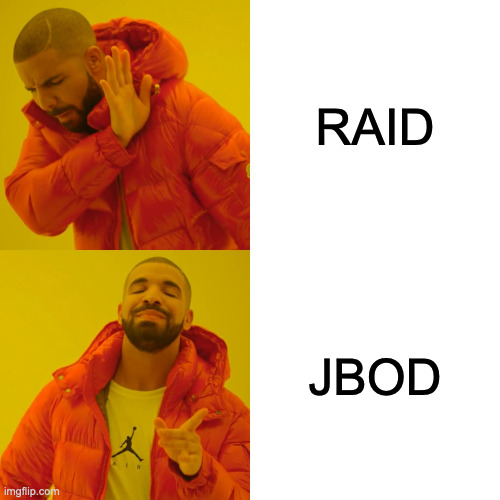
\includegraphics[width=0.5\textwidth]{images/jbod.jpg}
\end{center}

This is the do-nothing approach.

Manual backups? 

\end{frame}


\begin{frame}
\frametitle{RAID 0}

Disk striping; no redundancy.

\begin{center}
	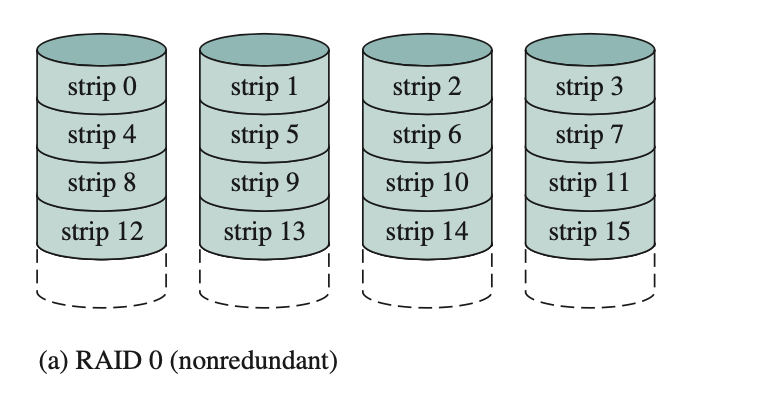
\includegraphics[width=\textwidth]{images/raid0.png}
\end{center}

Some use cases for it...

\end{frame}


\begin{frame}
\frametitle{RAID 1}

Mirroring

\begin{center}
	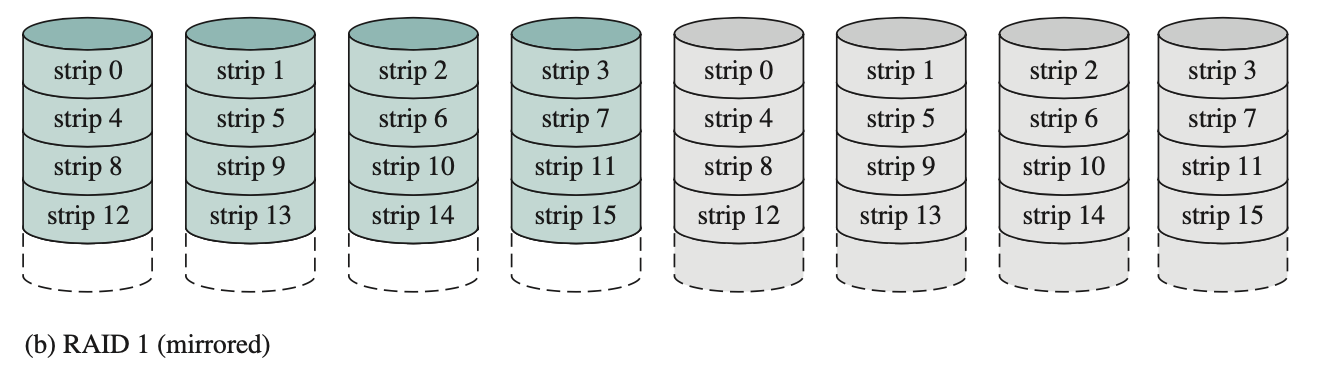
\includegraphics[width= \textwidth]{images/raid1.png }
\end{center}

\end{frame}


\begin{frame}
\frametitle{RAID 2}

Bit Parity

\begin{center}
	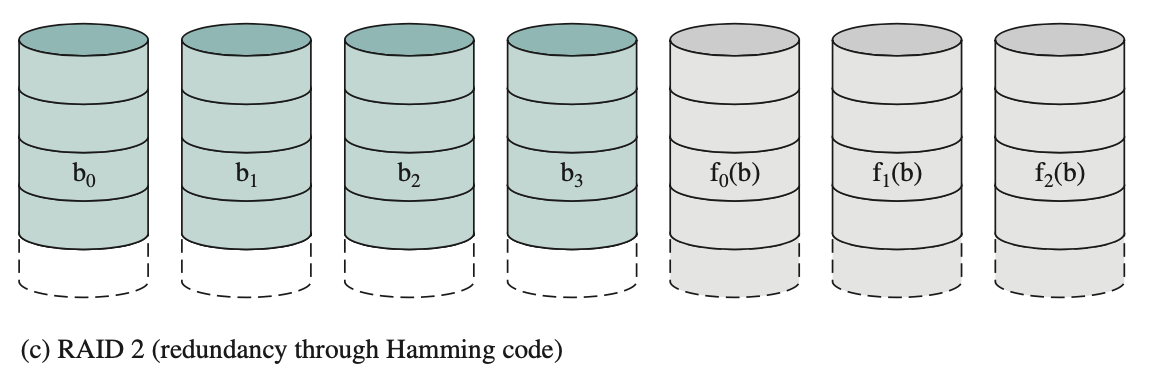
\includegraphics[width= \textwidth]{images/raid2.png }
\end{center}


\end{frame}


\begin{frame}
\frametitle{RAID 3}

Byte Parity

\begin{center}
	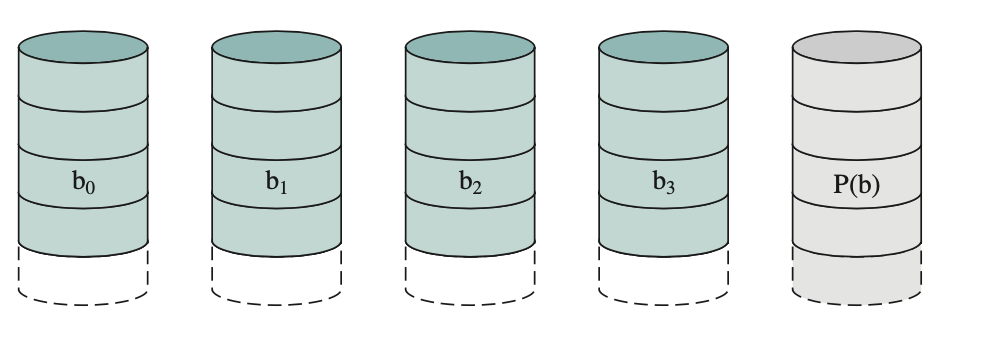
\includegraphics[width= \textwidth]{images/raid3.png}
\end{center}


\end{frame}


\begin{frame}
\frametitle{RAID 4}

Block Parity

\begin{center}
	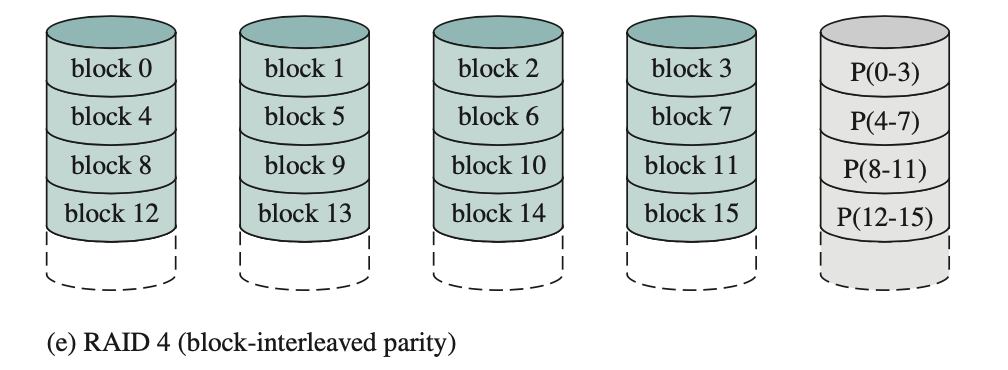
\includegraphics[width= \textwidth]{images/raid4.png}
\end{center}


\end{frame}


\begin{frame}
\frametitle{RAID 5}

Distributed Block Parity

\begin{center}
	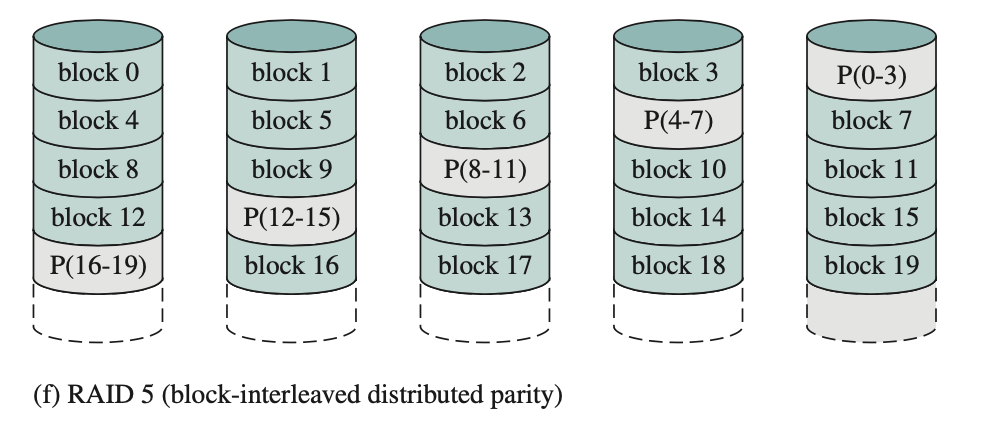
\includegraphics[width=\textwidth]{images/raid5.png}
\end{center}

\end{frame}


\begin{frame}
\frametitle{RAID 6}
Like RAID 5 but can survive more disk failures.

\begin{center}
	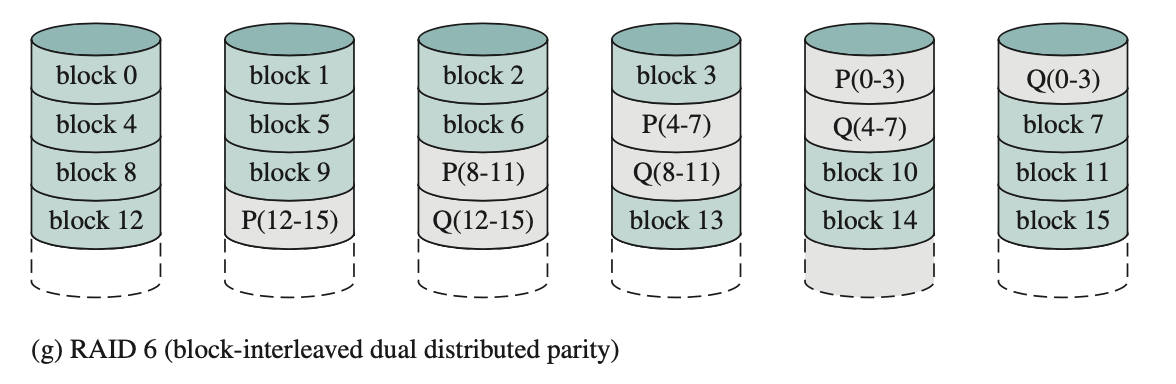
\includegraphics[width= \textwidth]{images/raid6.png}
\end{center}

\end{frame}


\begin{frame}
\frametitle{Combining Levels}

here are a number of ways that RAID may be combined, such as RAID 01, 10, 50... 

These are best thought of as being something like 1 + 0 rather than ten, because what we're doing is combining both these things at two different levels. 

\end{frame}

\begin{frame}
\frametitle{Combining Levels}

\begin{center}
	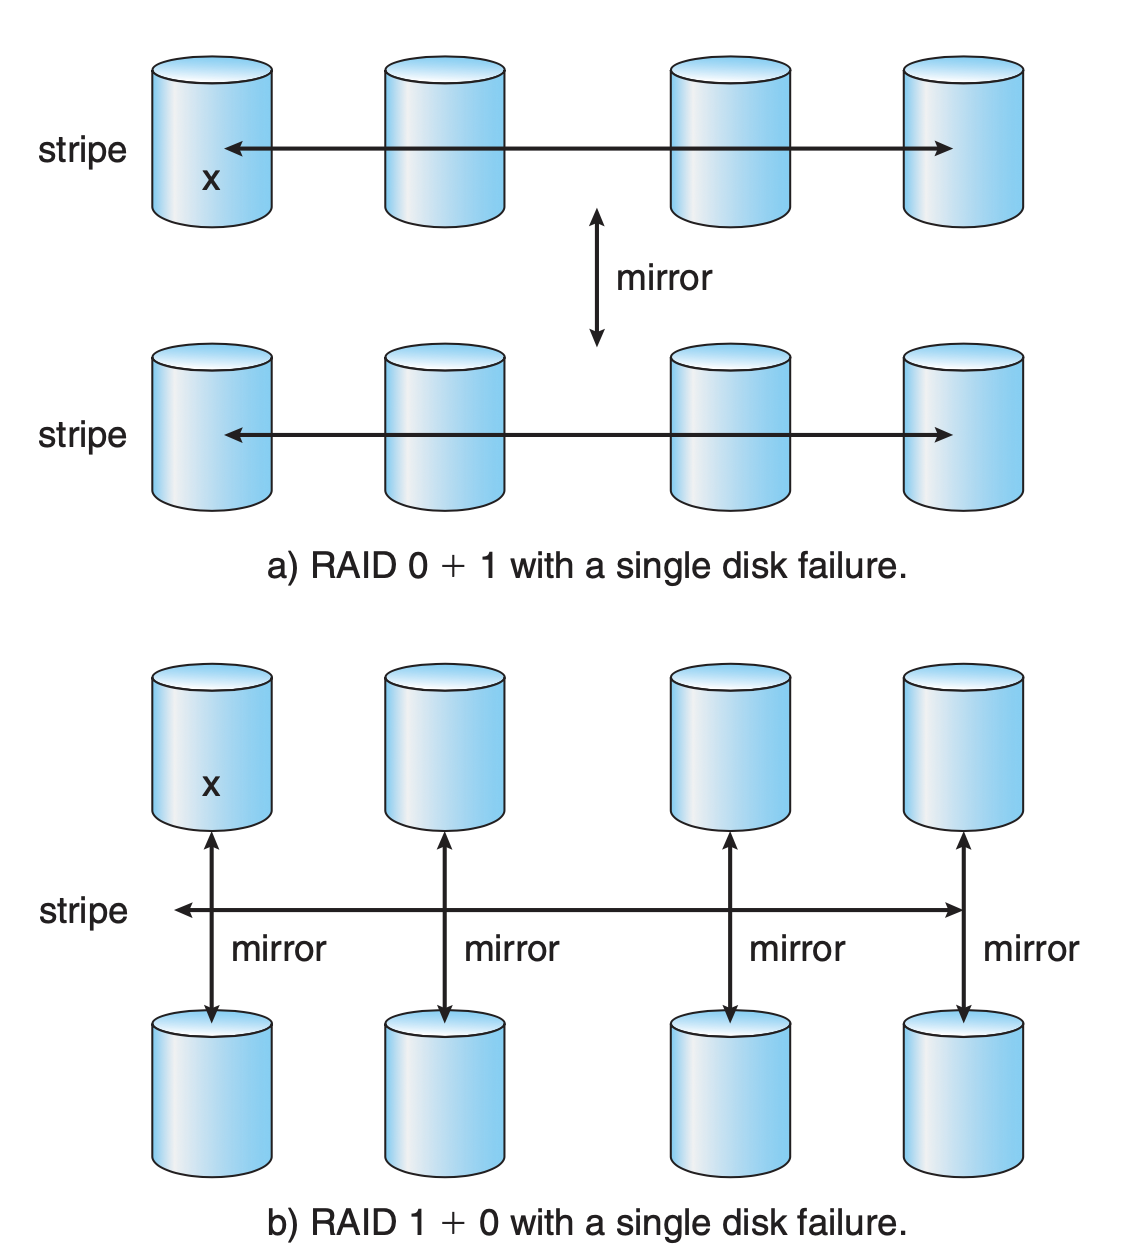
\includegraphics[width=0.5\textwidth]{images/raid10-01.png}
\end{center}


\end{frame}


\begin{frame}
\frametitle{Choosing the Right Level}

\begin{itemize}
	\item How critical is it that data is not lost?
	\item What is the budget?
	\item How important is performance?
	\item Do we need to be able to carry on in the event a disk dies?
	\item Are rebuild times important?
\end{itemize}

\end{frame}


\begin{frame}
\frametitle{Choosing the Right Level}

No one-size-fits-all answers.

RAID 2, 3, 4 not very popular...

Choose what makes sense!

\end{frame}





\end{document}

